% File: tikz2pdf-usage.tex
% Author: Marcin Szewczyk
% Title: Generating PDF Figures from TikZ Code -- Use Case

\documentclass[a4paper,11pt]{article}

% --- Encoding & language ---
\usepackage[T1]{fontenc}
\usepackage[utf8]{inputenc}
\usepackage[polish,english]{babel}

\newif\ifenglish
%\englishfalse
\englishtrue

\AtBeginDocument{
	\ifenglish
	\selectlanguage{english}
	\else
	\selectlanguage{polish}
	\fi
}

% --- Layout ---
\usepackage[left=18mm,right=18mm,top=18mm,bottom=18mm]{geometry}

% --- Graphics and subfigures ---
\usepackage{graphicx}
\usepackage{subcaption}

% --- Metadata ---
\title{
	\ifenglish
	Generating PDF Figures from TikZ Code -- Use Case
	\else
	Generowanie rysunków PDF z kodu TikZ -- przykład użycia
	\fi
}
\author{Marcin Szewczyk}
\date{\today}

\setlength{\fboxsep}{20pt} % odległość ramki od rysunku
\setlength{\fboxrule}{1pt} % grubość ramki

\addto\captionsenglish{\renewcommand{\figurename}{Fig.}}
\addto\captionspolish{\renewcommand{\figurename}{rys.}}

\begin{document}
	
	\maketitle
	
	\begin{center}
		\ifenglish
		Example of including graphics from PDF files generated from TikZ code: Fig.~\ref{fig:1}, \ref{fig:2}, \ref{fig:3}.
		\else
		Przykład wstawiania grafiki z plików PDF wygenerowanych z kodu TikZ: rys.~\ref{fig:1}, \ref{fig:2}, \ref{fig:3}.
		\fi
	\end{center}
	
	\begin{figure}[ht]
		\centering
		\fbox{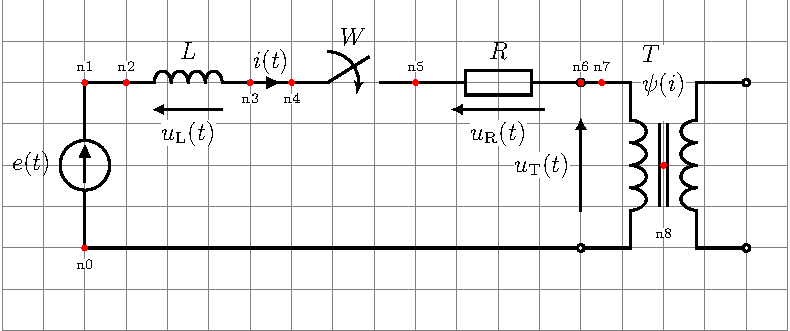
\includegraphics[width=0.6\textwidth]{./output/tikz2pdf-crop-1.pdf}}
		\caption{
			\ifenglish
			PDF file with grid and nodes
			\else
			Plik PDF z siatką pomocniczą i węzłami
			\fi
		}
		\label{fig:1}
	\end{figure}
	
	\begin{figure}[ht]
		\centering
		\fbox{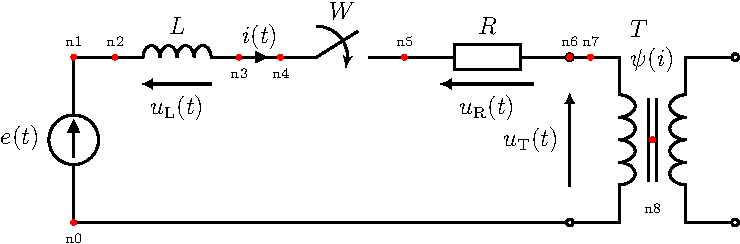
\includegraphics[width=0.6\textwidth]{./output/tikz2pdf-crop-2.pdf}}
		\caption{
			\ifenglish
			PDF file with nodes
			\else
			Plik PDF z węzłami
			\fi
		}
		\label{fig:2}
	\end{figure}
	
	\begin{figure}[ht]
		\centering
		\fbox{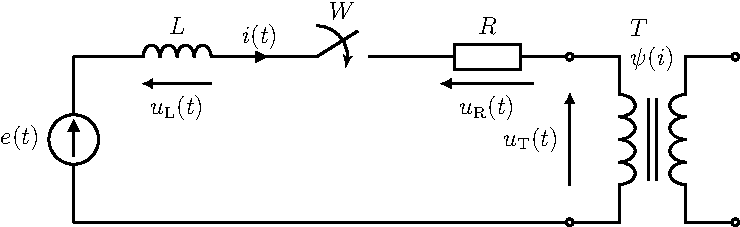
\includegraphics[width=0.6\textwidth]{./output/tikz2pdf-crop-3.pdf}}
		\caption{
			\ifenglish
			Final PDF
			\else
			Końcowy PDF
			\fi
		}
		\label{fig:3}
	\end{figure}
		
\end{document}
